\documentclass[10pt,a4paper]{article}
\usepackage[utf8]{inputenc}
\usepackage[T1]{fontenc}
\usepackage{amsmath}
\usepackage{amsfonts}
\usepackage{amssymb}
\usepackage{graphicx}
\usepackage[noabbrev]{cleveref}
\usepackage{mathrsfs}
\usepackage{mathtools}
\usepackage{enumerate}
\usepackage[left=2.00cm, right=2.00cm, top=2.00cm, bottom=2.00cm]{geometry}

%%
\linespread{1.5}
\newcommand{\Normal}{\operatorname{Normal}}
\newcommand{\Gmma}{\operatorname{Gamma}}
\newcommand{\Lognormal}{\operatorname{Lognormal}}

%Import the natbib package and sets a bibliography  and citation styles
\usepackage[round, sort, numbers]{natbib}
\setcitestyle{square}
\bibliographystyle{unsrtnat}
%%

\title{A Framework For Considering Costs and Benefits of Additional Complexities in Personalized Medicine \\
		\large Working Title Need a New One}

\author{Demetri Pananos, Dan Lizotte}

\date{}


\begin{document}
	\maketitle

	\section{Introduction}

Personalized medicine has four goals: 1) to identify drugs for which between-subject variability in effectiveness or toxicity is a key issue for effective treatment, 2) to identify predictors which may explain this variability, 3) to decide on the right dose of the right drug by considering these factors, and 4) prevent adverse reactions to drugs \cite{morse2015personalized}.  Progress in all four goals has accelerated within the last decade. As an example, recent studies on DPYD genotype testing prior to starting fluoropyrimidine-based chemotherapy showed promise in preventing adverse events, making good arguments for integration of DPYD genotype testing into standard of care practices \cite{wigle2019prospective}. Despite this progress, personalized medicine still faces several barriers to widespread adoption, including economic burden, patient burden, and expertise burden required for new methods of personalization.


Personalized medicine reduces costs to the healthcare system by identifying patients who are at greater risk for adverse events or dose adjustments, thereby optimizing safety.  If the patient does not undergo an adverse event, then this ultimately saves the healthcare system the cost of the hospital stay \cite{looff2016economic}.  More ambitiously, personalized medicine has the potential to save the healthcare system costs by more effectively using resources \cite{shabaruddin2015economic}. The cost of instruments, technicians, and leadership required to operate a personalized medicine clinic are high burden, and it is not yet clear if personalized medicine is sufficiently cost effective to offset operating costs in all circumstances \cite{kasztura2019cost}.  In their 2019 scoping review of personalized medicine cost effectiveness, Kasztura et. al \cite{kasztura2019cost} found that willingness-to-pay thresholds vary wildy from country to country (citing that cost per quality adjusted life year for some modes of personalized medicine range from \$20, 000 USD per quality adjusted life year in for studies in Europe and the United Kingdom to \$200,000 USD per quality adjusted life year for studies in the United States).  This high variability in cost effectiveness means the burden required for start up may result in a positive return on investment in some areas but not others. This variability should prompt would be adopters to more closely examine if taking on the initial burden is worth the result.


% beef up here
% Examples.  Identifty clear examples from the literature around diagnostics?
The dominant perspective on personalized medicine focuses on the use of clinical and physioligical information (including biomarkers, genotyping, and diagnostic tests) as a means of optimizing treatments, but largely ignore needs, constraints, and utilities of the patient \cite{rogowski2015concepts, di2017personalized}. Patients can be burdened by frequent followup for clinical measurement (as in the case with Warfarin), be burdended by costly expenses related to obtaining care, or may be more risk adverse/tolerant than the ``typical'' patient. As an example, transportation has been found to be a large financial burden for patients recieving cancer treatment \cite{houts1984nonmedical}, and continues to burden patients, with a 2020 study finding that the cost of parking alone can climb as high as \$1600 over the course of treatment in the United States \cite{lee2020assessment}.  Additional visits to a clinic have the potential to further burden patients by requiring them to miss a day of work, and find means of childcare during their absence (if neccesary). Incorporating patient preferences and reducing the burden of personalization on the patient can result in sustained adherence \cite{elliott2008understanding}, thereby increasing effectiveness and further preventing adverse events.


% FInd some machine learning cautinary tales

An additional expertise burden is added as machine learning (used interchangeably with the term “artificial intelligence”) is adopted into personalized medicine initiatives.  Cutting edge machine learning models for prediction or decision making can be prohibitively burdensome to implement effectively. Failure to do so may result in pernicious bias inadvertently affecting subpopulations, as was found to be the case in algorithms for credit scoring \cite{barocas2016big}, crime prediction \cite{lum2016predict}, and hiring \cite{ajunwa2020paradox}.  A 2019 study found an instance of this bias in a widely used risk scoring algorithm in healthcare \cite{obermeyer2019dissecting}, demonstrating that despite the best intentions of those involved, the use of a model can lead to worse rather than better care if investigators are not careful in considering what sorts of bias may be present in the data used to train these models.  Implementation of new approaches and methods requires the close collaboration of experts in data science  with physicians, domain experts, and other stakeholders.  Close collaboration should allow for domain experts to identify what kinds of biases the data might have, and for data science experts to implement methods to help ammeliorate that bias (or to admit the data are not fit for purpose).  The result of iterating on this collaborative process (wherein domain experts help inform the appraoches methodologists take, and the methodologists provide model checks which help domain experts decide if decisions from the model are reasonable or suspicious) is a model which more closely aligns with domain expertise, a model which is sufficiently flexible to capture the true data generating mechanism, an effective use of data, a more transparent modelling process, and calibrated expectations surrounding algorithms and their abilities \cite{frohlich2018hype}.  Presently, this form of collaboration between methodologists and domain experts is not the norm, with developement of machine learning solutions in healthcare bdeing developed in silos \cite{wiens2019no}.

These burdens may be surmountable for some, but the question then turns to if the result is worth the expense.  Answering that question is difficult without an idea how the additional burden of collecting data, or implementing new algorithms, will benefit the clinic or the patient subject to inherent constraints. 

 In this study, we present a new framework for helping practitioners interested in implementing personalized medicine to answer a) If the burden of personalization could result in more favorable outcomes for their population of patients, b) how working around patient burden (such as coming into the clinic for fewer measurements) may change effectiveness, and c) if more complex models for personalization can lead to better effectiveness. For our case study, we fit a Bayesian model to existing data on the pharmacokinetics of apixaban.  The resulting Bayesian model is used to generate synthetic pharmacokinetic data for use in experiments to compare different forms of personalization. Treating personalization as a dynamic treatment regime, we propose six policies, each increasing in complexity and clinic/patient burden, for personalizing doses of apixaban with the goal of keeping blood serum concentrations within a desired range for as long as possible. Under the assumption that the fitted Bayesian model can produce similar data to what might be observed in the future from new patients, we can make inferences as to how different policies for personalizing doses may improve upon one another, and compare if the additional burden of implementing a more complex or costly form of personalization can generate a more desirable outcome for the patient or healthcare provider.  

We begin with an overview of dynamic treatment regimes.  We then describe how to estimate an optimal dynamic treatment regime  by combining Bayesian pharmacokinetic modelling with Q-learning.  We then present our case study, beginning with the details of the Bayesian model we use to fit the real pharmacokinetic data, and present model fit diagnostics to argue that our model is satisfactory for generating synthetic data for use in our simulations. We then present and discuss the results of our simulation in light of the burden presented to a clinic to implement personalized medicine, and how this framework can be integrated to answer questions such as if personalization can produce a positive return on investment, how burdening the patient with an additional clinic visit will improve the clinic's understanding of how to treat that patient, and if using a more advanced mode of personalization will result in more favortable health outcomes.
%Given these three types of burden, want to assess if it is worth doing or not.
% Concrete examples from the three burdens 

	\section{Dynamic Treatment Regimes}



In this section, we discuss the theory of dynamic treatment regimes and how personalization can be thought of as a dynamic treatment regime.  We describe our experiments in the context of dynamic treatment regimes and introduce our reward function.

\subsection{Trajectories}

Our goal is to find the dose or sequences of doses for a subject to keep their blood serum concentration within a desired range for as long as possible given the constraints: a) subject’s blood serum concentrations cannot be measured very frequently, and b) we are limited to pre-dose clinical measurements to make our initial dosing decision.  The theory of dynamic treatment regimes and statistical reinforcement learning offers a framework through which to understand our problem and construct one possible solution.

A dynamic treatment regime (DTR) is a sequence of decision rules for adapting a treatment plan to the time-varying state of an individual subject \cite{chakraborty2013statistical}. In DTRs, and their cousin topic in computer science \textit{reinforcement learning}, an agent (often thought of as a robot in reinforcement learning, but within medicine sometimes thought of as a physician’s computerized decision support system) interacts with a system for a number of stages. At each stage, the agent receives an \textit{observation} of the system and then decides which \textit{action} to take.  This action will result in an observed \textit{reward} which is followed by a new observation of the system after it has been impacted by the action.  This cycle of observation, action, reward then repeats, with the agent aiming to take actions which yield the largest total reward.

Key to our DTR is the concept of a \textit{trajectory}. Define a stage to be a triple containing an observation, chosen action, and resulting reward. Let $O_i$ denote an observation at the ith stage, $ A_i $ be the action at the $ i^{th} $ stage, and $ Y_i $ denote the reward at the $ i^{th}$ stage, denoted in capital letters when considering the observation, action, and reward as random variables.  A  trajectory is then the tuple $ (O_1, A_1, O_2, A_2,  \cdots, O_K, A_K, O_{K+1})$.  Following notation by Chakraborty and Moodie \cite{chakraborty2013statistical}, we will denote a system’s history at stage $ j $ as $ H_j = (O_1, A_1, O_2, A_2, \cdots , O_{j-1}, A_{j-1}, O_j) $.  The reward at stage j is then a function of the system’s history, the action taken, and the next observation $ Y_j = Y_j(H_j, A_j, O_{j+1}) $.

\subsection{Policies, Value Functions, and Q-Learning}

A deterministic policy $ d = (d_1, \cdots, d_k) $ is a vector of decision rules each which take as input the system’s history and output an action to take. The stage $ j $ value function for a policy $ d $ is the expected reward the agent would receive starting from history $ h_j  $(here in lower case since it is an observed quantity) and then choose actions according to $ d $ for every action thereafter.  The value function is written as

\begin{equation}
	V^d_j(h_j) = E_d\left[ \sum_{k=j}^K Y_k(H_k, A_k, O_{k+1}) \Bigg\lvert H_j = h_j\right] \>.
\end{equation}

\noindent Here, the expectation is computed over the distribution of trajectories. Importantly, the stage $ j $ 
value function can be decomposed into the expectation of reward at stage $ j $ plus the stage $ j+1  $ value function  \cite{chakraborty2013statistical}

\begin{equation}
V^d_j(h_j) = E_d\left[Y_j(H_j, A_j, O_{j+1} + V^d_{j+1}(H_{j+1}) \vert H_j = h_j\right] \>.
\end{equation}


\noindent The optimal stage $ j  $ value function is the value function under a policy which yields maximal value.  Mathematically, 

\begin{equation}
V^{opt}_j(h_j) = \underset{d \in \mathscr{D}}{\mbox{max}} V^d_j(h_j)
\end{equation}

\noindent A natural question is “what policy maximizes the value?”. Estimating such a policy can be achieved by estimating the optimal Q function \cite{chakraborty2013statistical}.  The optimal Q function at stage $ j $ is a function of the system’s history $ h_j $ and a proposed action $ a_j $,

\begin{equation}
 Q_j^{opt} = E \left[ 
 Y_j(H_j, A_j, O_{j+1}) + V^{opt}_{j+1}(H_{j+1}) \lvert H_j = h_j, A_j = a_j
 \right]
\end{equation}

Note that the optimal Q function has similar form and interpretation to the optimal value function (namely, it is the expected reward starting at stage $ j $ but with the added condition that we take action $ a_j $ and then follow the optimal policy thereafter). Due to the decomposition of the reward function at stage $ j $, estimation of the optimal Q function can be performed by choosing the action which yields the largest reward at each stage assuming we act optimally in the future.  Below, we describe how we choose optimal actions using a posterior distribution of a subject’s pharmacokinetics.

\subsection{Experimental Design In Terms of Stages of a DTR}

In our experiments, we develop a DTR for selecting the best dose for keeping a patient’s blood plasma concentration within a desired range. Here, we present details of the experimental design in the DTR framework, leaving simulation details (including how the data were simulated) for our methods section.

Our experiment consists of 1000 simulated subjects taking a dose of apixaban once every 12 hours with perfect adherence for a total of 10 days.  Sometime in the second 12 hour period on the fourth day (between 108 and 120 hours after the initial dose), we have the opportunity to measure  the simulated subject’s blood concentration, should our policy allow for it.  At the start of the fifth day, the dose is adjusted based on all the pre-dose clinical measurements plus the observed concentration. The dose will be adjusted so as to attempt to maximize the time spent between 0.1 mg/L and 0.3 mg/L. Thus, our DTR consists of two stages (the first five days, and the latter five days), however the size of the range may be adapted for different scenarios. We choose this range as it is not so narrow that even optimal doses perform poorly, but not so wide that any dose can achieve high reward. 

In terms of the DTR, the system is the patient for whom a dose is selected, the actions correspond to selection of dose sizes, and the reward is the proportion of time spent within the desired concentration range. The trajectories we will use to estimate the optimal Q functions are of the form

\begin{equation}\label{key}
O_1, A_1, Y_1, O_2, A_2, Y_2, O_3
\end{equation}

\noindent The interpretation of a given trajectory is:
\begin{itemize}
	\item $ O_1 $ is any pre-dose clinical measurements of the subject.  In our experiments, we consider age in years, renal function (as measured by serum creatinine in mMol/L), weight in kilograms, and dichotmous biological sex (dummy coded so that male=1 and female=0).  We choose these variables as they are known to affect the pharmacokinetics of apixaban \cite{byon2019apixaban}.  
	\item $ A_1 $ is dual action of initial dose to provide the subject plus a time in the future at which to measure the subject’s blood serum concentration.
	\item $ Y_1 $ is the proportion of time spent within the concentration range in the first five days.
	\item $ O_2 $ is the pre clinical measurements of the subject plus the observed concentration made on the fourth day.
	\item $ A_2 $ is the dose adjustment
	\item $ Y_2 $ is the proportion of time spent within the concentration range in the last five days after the dose adjustment.
	\item $ O_3 $ would be pre-dose clinical measurements, the observed concentration made on the fourth day, and the next concentration measurement, were it to be made. As we examine just the two actions $ A_1 $ and $ A_2 $, we do not make use of $ O_3 $ but include it here to adhere with our definition of trajectories above.
\end{itemize}

The reward function we use depends on the subject’s true latent concentration. Let $ c_j j=1...K $ be the $ j^{th}$ latent concentration value at time $ t_j $.  The reward function is 

\begin{equation}
Y(c_1, c_2, \cdots, c_k) = \dfrac{1}{k}\sum_{j=1}^K \mathbb{I}(0.1 < c_j < 0.3)
\end{equation}

\noindent Here, $ \mathbb{I} $ is an indicator function returning 1 if the argument is true, and 0 else.  To leverage off-the-shelf optimization tools, we approximate this reward function with a continuously differentiable function, namely
\begin{equation}
Y(c_1, c_2, \cdots, c_k) = \dfrac{1}{k}\sum_{j=1}^K \exp\left( - \left[ \dfrac{c_j-0.15}{0.05} \right]^{2\beta} \right)
\end{equation}

\noindent Here, $ \beta $is a positive integer.  For sufficiently large beta, our approximation becomes arbitrarily close to our intended reward function.  In practice we set beta=5 to balance between good approximation of our intended reward and vanishing gradients impeding our optimization. We suppress the dependence on the history in the definition of the reward as the reliance on the history is implicit.  The reward depends on the latent concentrations which depend on previous doses (actions) and potentially on the previous dose measurements (observations of the system).

Our stage 2 optimal Q function is then

\begin{equation}
Q_{2}^{o p t}\left(H_{2}, A_{2}\right)=E\left[Y\left(c_{j+1}, c_{j+2}, \cdots, c_{j+n}\right) \Bigg\vert H_{2}, A_{2}\right] \>,
\end{equation}

\noindent and our stage 1 optimal Q function is

\begin{equation}
Q_{1}^{o p t}\left(H_{1}, A_{1}\right)= E \left[Y\left(c_{1}, c_{2}, \cdots, c_{j}\right)+\max _{a_{2}} Q_{2}^{o p t}\left(H_{2}, a_{2}\right) \Bigg\vert H_{1}, A_{1}\right]
\end{equation}

We seek to maximize the stage 1 optimal Q function to learn the optimal policy for dosing subjects under the constraint we can measure them at most once and are limited to the aforementioned pre-dose clinical variables.  The interpretation of stage 1 optimal Q function is as follows:\textit{ Given the pre-dose clinical variables of the subject and a proposed initial dose and measurement time, the stage 1 optimal Q function gives the proportion of time the subject’s blood serum concentration is between 0.1mg/L and 0.3mg/L assuming that we provide the subject with the best dose possible at the start of the $ 5^{th} $ day.}  The actions $ A_1 $ and $ A_2 $ which maximize these functions constitute the optimal policy.

The concentration values $ c_j $ in the optimal Q functions are latent, meaning we have no direct access to them in practice. Furthermore, obtaining measurements with high enough frequency so that the reward is faithfully estimated would be too burdensome on the patient. What is left to explain is how these concentrations are computed. In the next section, we describe how we use a Bayesian model  to obtain latent concentration predictions and compute the required expectations.

	\section{Bayesian Models of Pharmacokinetics}

In order to estimate the optimal Q functions, we need to be able to predict how a subject’s concentrations respond to any given dose.  These predictions can be passed to the reward function to compute the values of $ Q_1 $ and $ Q_2 $. Bayesian models of pharmacokinetics are capable of providing distributions of concentrations and can account for pre-dose clinical variables, as we will describe.  The model we construct takes as inputs pre-dose clinical variables (age, sex, weight, and creatinine) and provides a distribution of plausible concentrations prior to seeing data.  We can pass these prior predictions to our Q function and determine what dose keeps the subject in range for the longest time prior to seeing any data.  Once we observe a concentration measurement from the subject, we can condition our model on that observation, and perform the optimization again to adjust the subject’s dose in light of new information.   For our experiments, we first fit a Bayesian pharmacokinetic model to real pharmacokinetic data collected by our colleagues in clinical pharmacology \cite{tirona2018apixaban} and then use the fitted model to simulate patients and make predictions for our experiments.

We extend a previously proposed one compartment Bayesian pharmacokinetic model \cite{pananos2020comparisons} to include fixed effects of covariates on pharmacokinetic parameters.  The model presented in \cite{pananos2020comparisons} is a hierarchical Bayesian model of apixaban pharmacokinetics, in which the clearance rate (L/hour), time to max concentration (hours), absorption time delay (hours), and ratio between the elimination and absorption rate constants (called alpha, a unitless parameter) are hierarchically modelled.  We extend that model by regressing the latent pharmacokinetic parameters on the aforementioned pre-dose clinical variables.

The model fit to real data, which we refer to as $ M1 $, is 

\begin{align}\label{model_M1}
	y_{i,j} &\sim \operatorname{Lognormal}  \left(  C_i(t_j)  , \sigma^2_y \right)  \\
	\sigma^2 &\sim \operatorname{Lognormal} \left( 0.1, 0.2 \right)\\	
	C_i(t_j) &= \begin{dcases}
	\frac{D_{i} \cdot F}{C l_{i}} \cdot \frac{k_{e, i} \cdot k_{a, i}}{k_{e, i}-k_{a, i}}\left(e^{-k_{a, i}\left(t_{j}-\delta_{i}\right)}-e^{-k_{e, i}\left(t_{j}-\delta_{i}\right)}\right) & t_j>\delta_i \\
	0 & \mbox{else}
	\end{dcases}\\
	k_{e,i} &= \alpha_i \cdot k_{a,i}\\
	k_{a,i} &= \dfrac{\log(\alpha_i)}{t_{max}\cdot(\alpha_i-1)}\\
	\delta_i &\sim \operatorname{Beta}(\phi, \kappa) \\
	\operatorname{logit}(\alpha_i) \vert \beta_\alpha, \sigma^2_\alpha &\sim \operatorname{Normal}(\mu_\alpha + \mathbf{x}_i^T \beta_\alpha, \sigma^2_\alpha)
\end{align}


	\section{Modes of Personalization}

Thus far, we have motivated personalization of dose sizes through Q learning.  Q learning is the most complex solution that could be implemented at this time, and its implementation in practice would be burdensome due to this complexity. This makes implementation of Q learning a tall order, especially considering alternative DTRs exist which are not as costly to implement. The cost of implementing Q learning may be worth paying if the benefit of Q learning over these other DTRs is substantial, but we need a framework in which to estimate the size of this benefit. 


Our study considers the following modes of personalization. Each one has different requirements in terms of computation, data needs, clinical overhead, and patient burden. Our study aims to understand, in this particular setting (apixaban with potential PK monitoring) what the relative benefits of these different modes might be in practice. It also presents a general framework for evaluating these different modes of personalization in other settings.  The six modes of personalization we consider are:

\begin{enumerate}[1)]
\item Dose selection using a hierarchical Bayesian model which does not incorporate subject covariates.  This model was presented in Pananos \& Lizotte \cite{pananos2020comparisons}.  We refer to this mode as the “No Covariate Model”.
\item 1) and conditioning the model on a single sample from the subject taken sometime in the final 12 hours before the half way point.  At the start of the fifth day, a new dose is selected and used for the remaining time.  We refer to this mode as “No Covariate + 1 Sample”.
\item Dose selection from M2.  A single dose is selected at the start of the regiment and is used throughout the 10 simulated days. We refer to this mode as “Covariate Model”.
\item 3) and conditioning the model on a single sample from the subject taken sometime in the final 12 hours before the half way point.  At the start of the fifth day, a new dose is selected and used for the remaining time. We refer to this mode as “Covariate model + 1 Sample”.
\item A two stage DTR, however the initial dose is the result of the procedure in 3).  The best time to sample the patient is then determined via Q learning. We refer to this mode as “Optimal Sampling Time”.
\item The two stage DTR we describe in the previous sections, estimated via Q learning.  We refer to this mode as “Q Learning”.

\end{enumerate}


We compare all methods on their achieved reward as well as the difference between the achieved reward and theoretically largest reward the reward we would achieve if we knew the pharmacokinetic parameters exactly).  Because we know the true latent pharmacokinetic parameters of the simulated subjects, we can optimize the reward with the known pharmacokinetics of the subject, thereby yielding the largest reward possible.


	\section{Results}
\subsection{Bayesian Model}



\begin{figure}
	\centering
	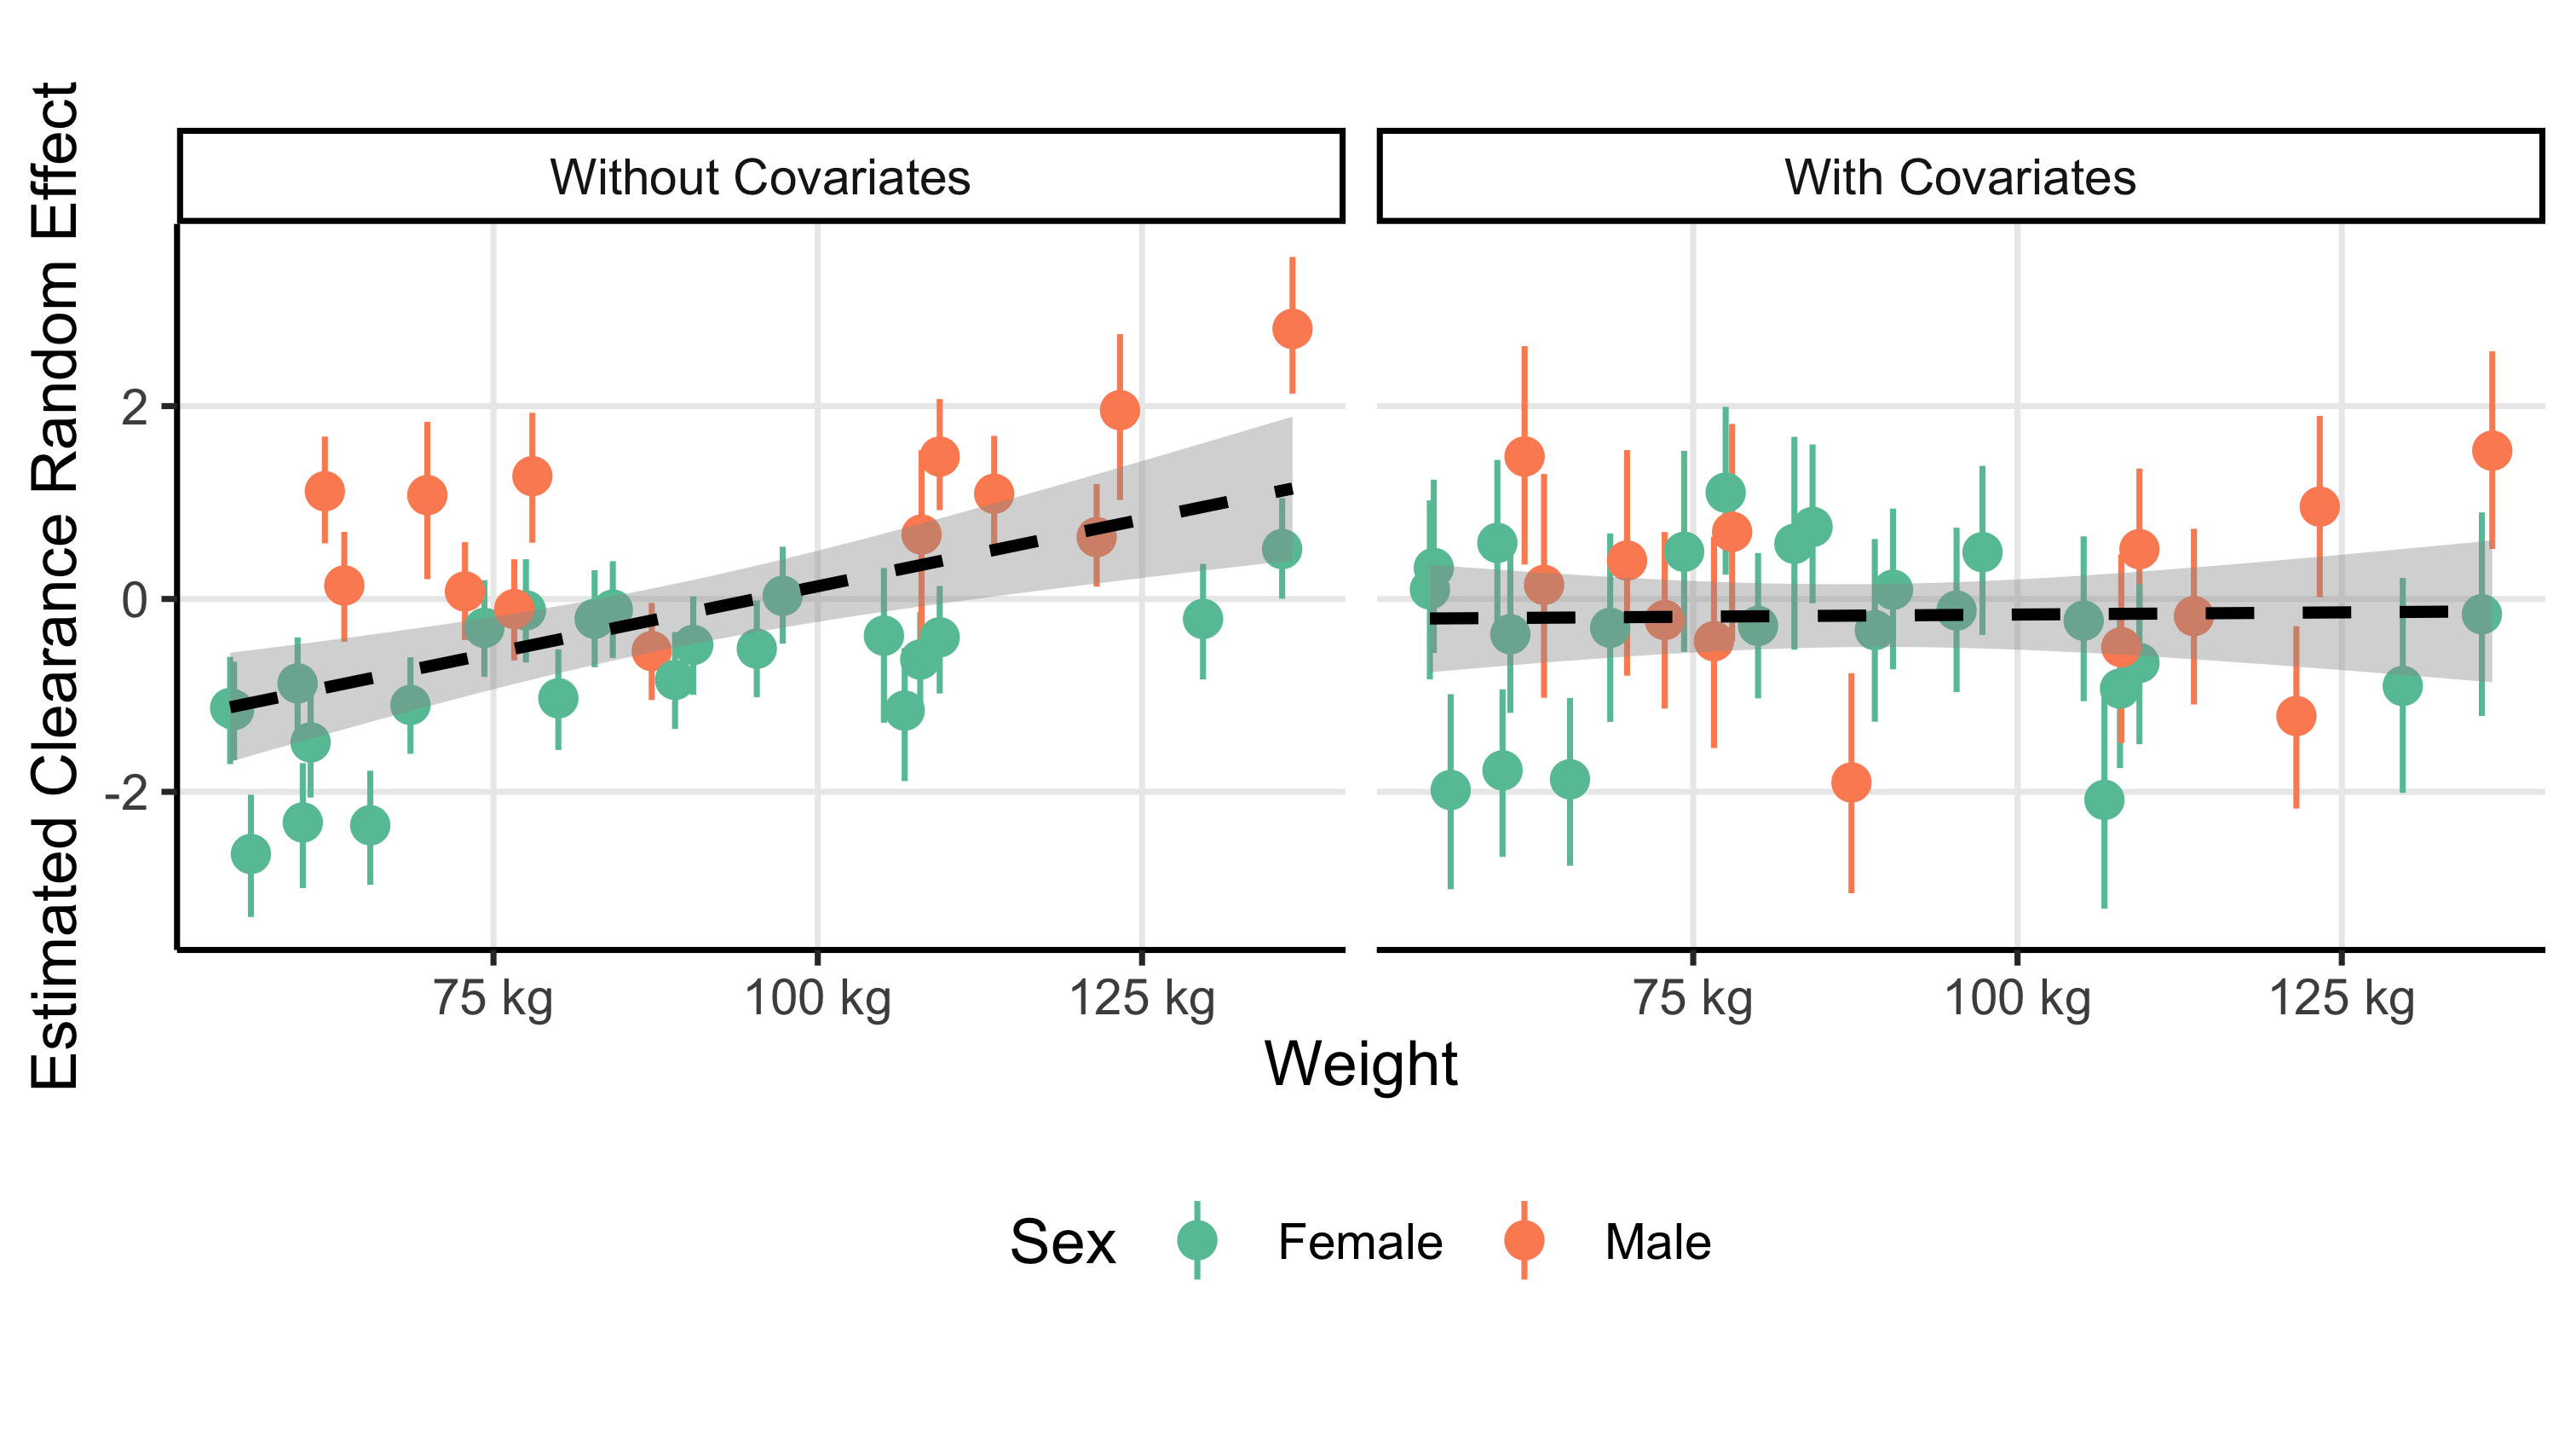
\includegraphics[width=\linewidth]{"figures/random_effects_change.png"}
	\caption{Random effects estimates for clearence rate $ Cl_i $and 95\% credible intervals (left).  Random effects estimates are colored by patient sex.  Prior to adjusting for covariates, a general trend in weight can be seen in the random effects.  Subjects who are heavier tend to have larger random effect, and males tend to have larger random effects than females of the same weight.  Patterns isuch as these indicate that weight and sex can be used to explain variation in the random effects.  After adjusting for sex and weight (right), the random effects have no discernable pattern.}
	\label{fig:randomeffectschange}
\end{figure}

In this section we present results of two different analyses.  We first assess the fit of our Bayesian model, as the model is crucial for our decision making experiments.  We then present the results of our decision making experiments.

We fit M1 to real pharmacokinetic data using Stan.  Stan monitors several markov chain diagnostics none of which detected problematic markov chain behavior, which indicates that Stan’s sampling algorithm was able to converge to the target distribution (0 divergences, all all Gelman-Rubin diagnostics<1.01, all effective sample size ratios  > 22\%).  

The inclusion of covariates in the model results in a better fit than excluding them. Shown in \cref{fig:randomeffectschange} are the estimated random effects for the clearance pharmacokinetic parameter of each subject as a function of weight.  Subject sex is indicated by color, the overall trend is shown in the black dashed line.  Failing to include subject sex and weight results in males having on average a larger random effect than females of the same weight, and heavier subejcts having a larger random effect than lighter subjects.  When covariates are added into the model, the variation in the random effects attenuates, resulting in closer alignment to model assumptions. A better fit to the data means data generate from the model may be closer aligned with the true data generating process.

Examining the posterior distributions of the regression coefficients provides further insight.  Subject weight increases the expected value of alpha (which is used to compute the elimination and absorption rates in the first order one compartment PK model.  The parameter $ \alpha $ is the ratio of how fast the drug exists the central compartment to how fast the drug enters the central compartment) as well as the time to max concentration.  There appears to be an effect of sex on $ \alpha $ (males have smaller alpha than females, meaning the drug leaves their central compartment slower or enters the central compartment quicker), however the uncertainty is large (estimated effect -0.2 on the logit scale, 95\% credible interval -0.54 to 0.15). See supplementary table X for a full summary of the regression coefficients.


\begin{figure}
	\centering
	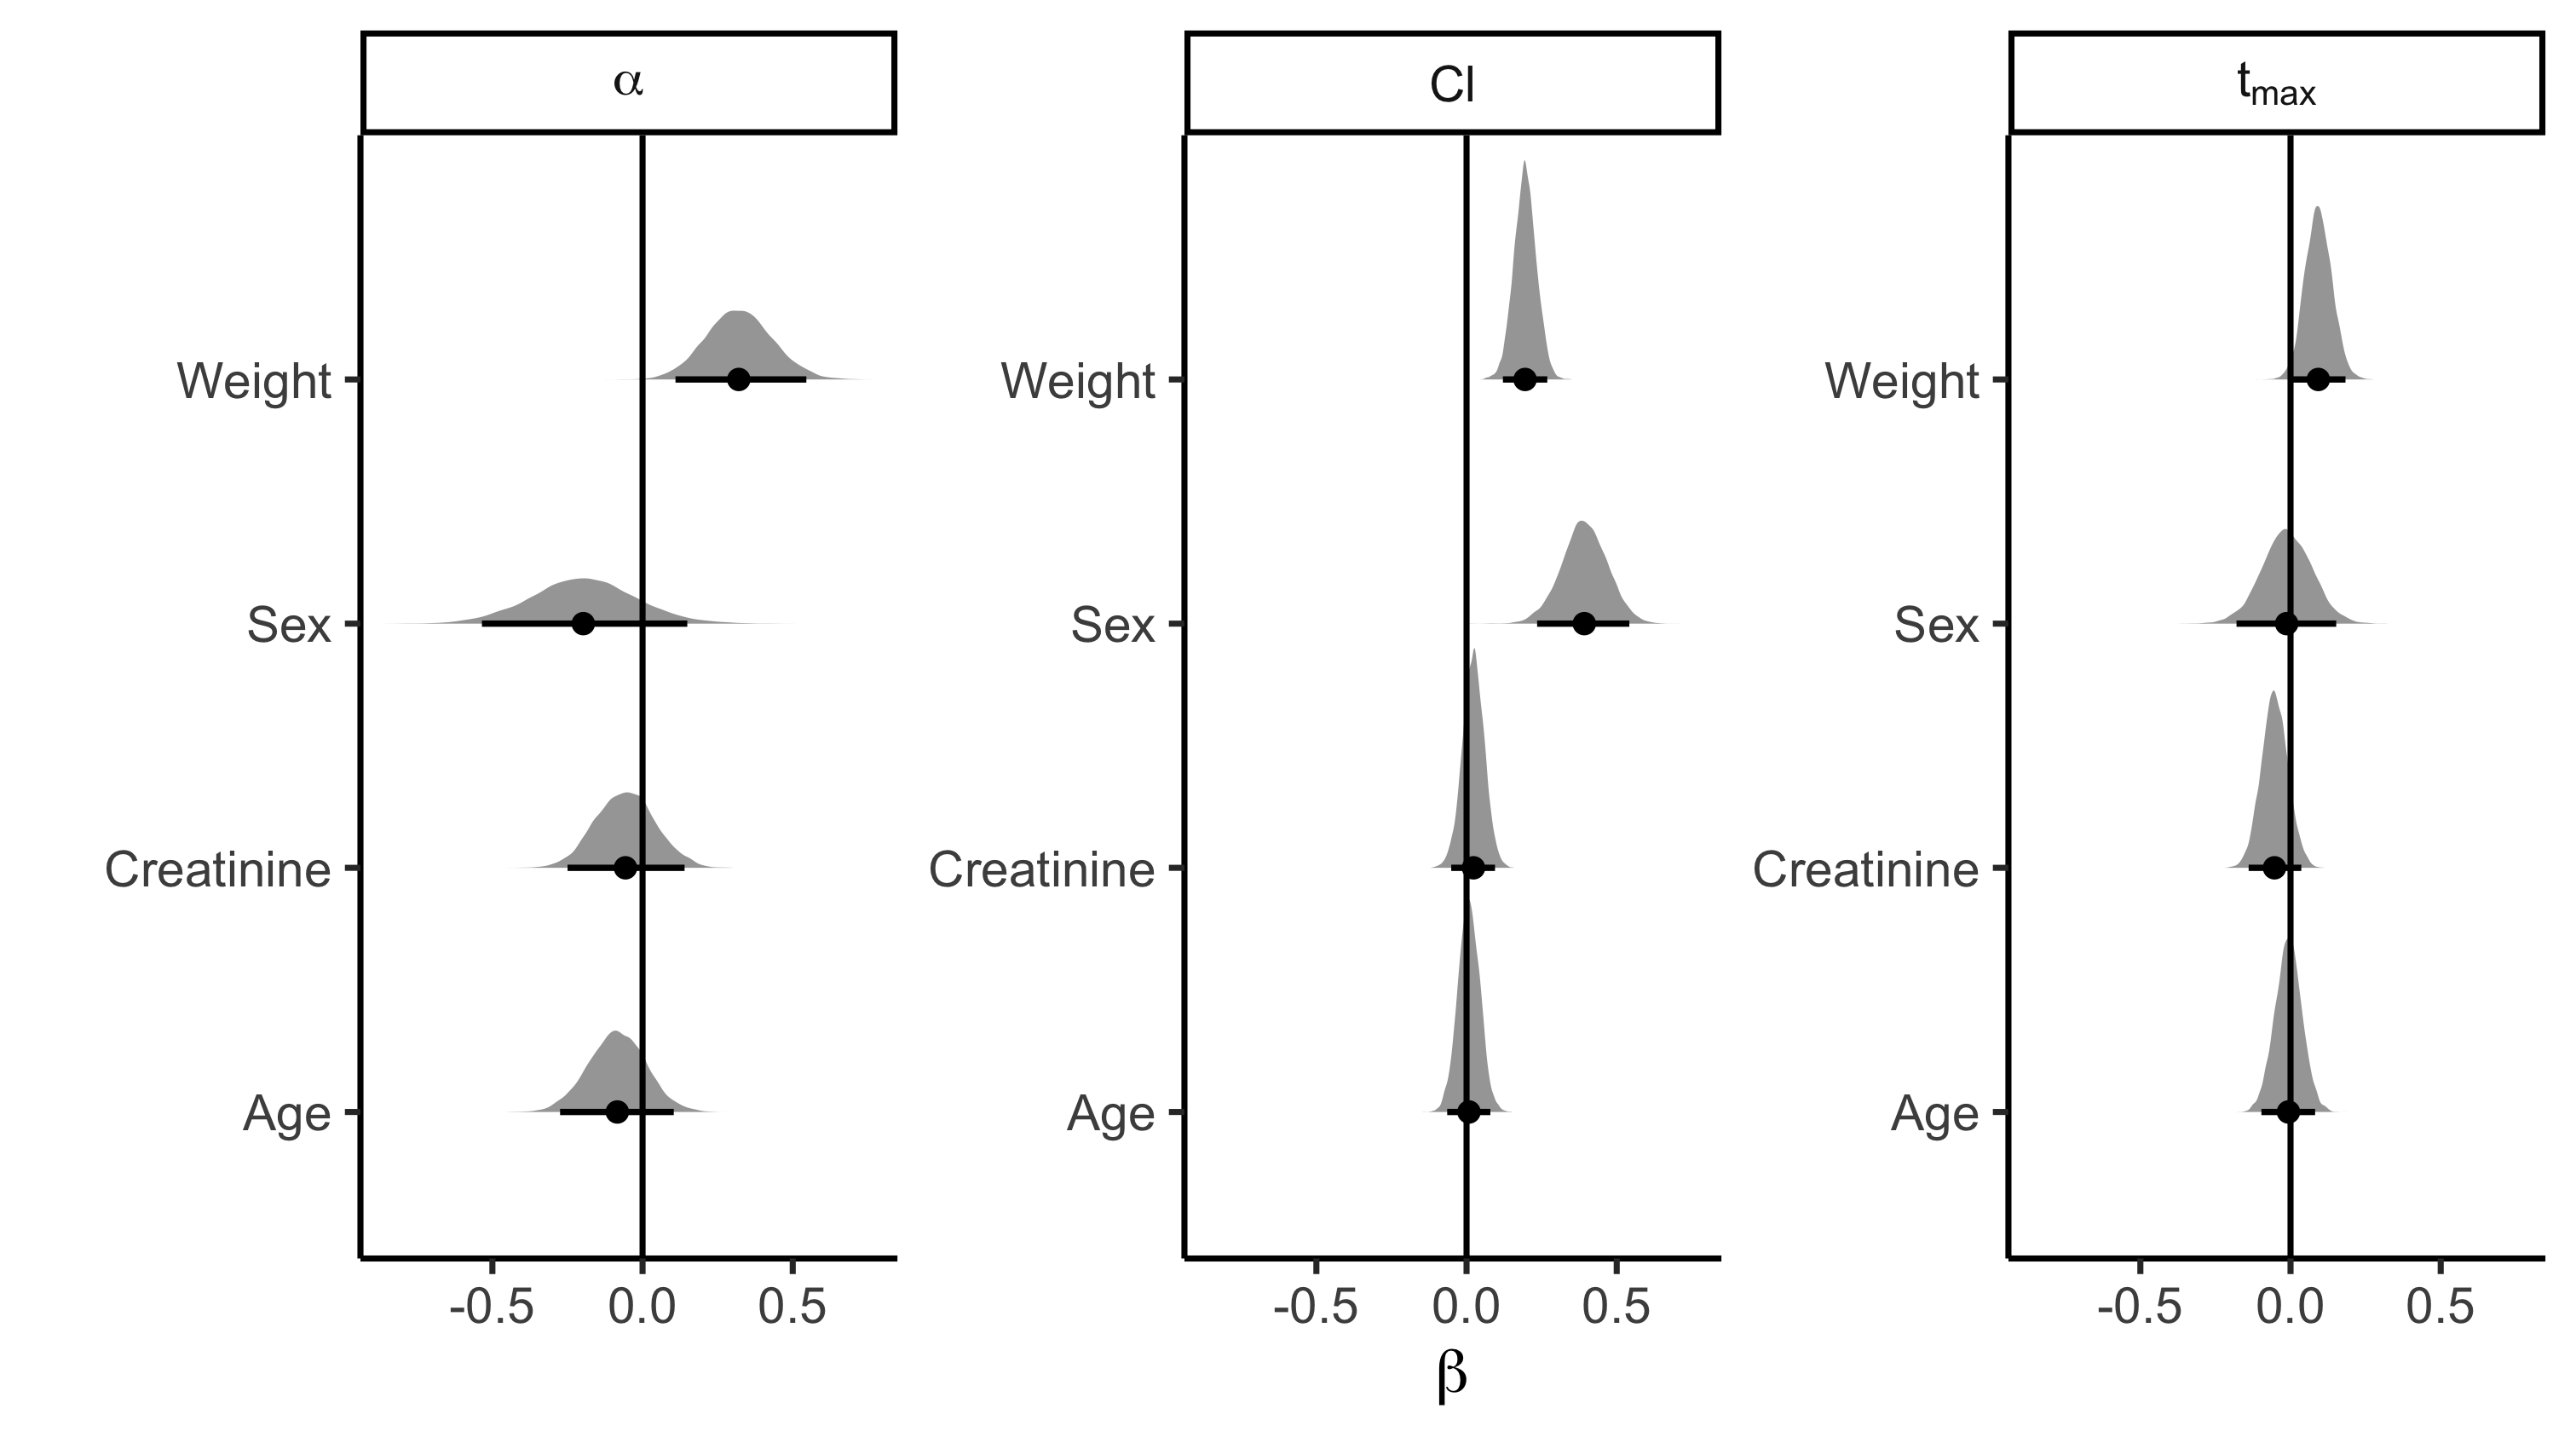
\includegraphics[width=1\linewidth]{figures/coef_vals}
	\caption{Posterior distributions of regression coefficients. Expectations are shown as black dots, 95\% credible intervals are shown as horizontal black lines.  Solid black vertical line is $\beta=0$ for reference.  Note, regression coefficients for $Cl$ and $t_{max}$ act multiplicatively (a one unit increase in weight leads to a change in $Cl$ of $\exp(\beta)$), while regression coefficients for $\alpha$ are interpreted on the log odds scale.}
	\label{fig:coefvals}
\end{figure}


Model training error sees a very small improvement.  Including subject covariates decreases model training error from 6.89 ng/ml to 6.84 ng/ml. Estimates of concentration uncertainty remain similar between the two models as well.  We conclude the inclusion of covariates in the model improves model inferences but does not improve the fit of the model to the data in any substantial way.  Either model would require additional validation prior to using in a predictive capacity.

\subsection{Simulation Results}

We consider 6 modes of personalization which range in the amount of information used in the decision process as well as burden placed on the patient and clinic, and burden of implementation.  We present the results of our simulation in figure X below in terms of difference between theoretically largest reward and reward achieved by the mode of personalization.  The results are ordered from least amount of information and burden (top) to most amount of information and burden (bottom).

Modes of personalization which use less information have a larger difference (i.e. yield smaller reward on average than what is theoretically possible).  The no covariate model (which uses no information about the subject) performs worst with a median difference of 0.19.  The distribution of differences for this mode is right skewed with some differences exceeding 0.95, meaning the subject could have been in range for nearly the entire time but the mode selected a dose which failed to put the subject in range. 

The use of covariates in the model nearly cuts the difference in half, achieving an average difference of 0.1 with smaller right skew.  There is a diminishing in the difference in rewards as additional burden is undertaken. Modes which use observed concentration information (Covariate Model + 1 Sample, Optimal Sampling Time, and Q Learning) lead to marginally more reward on average.


\begin{figure}
	\centering
	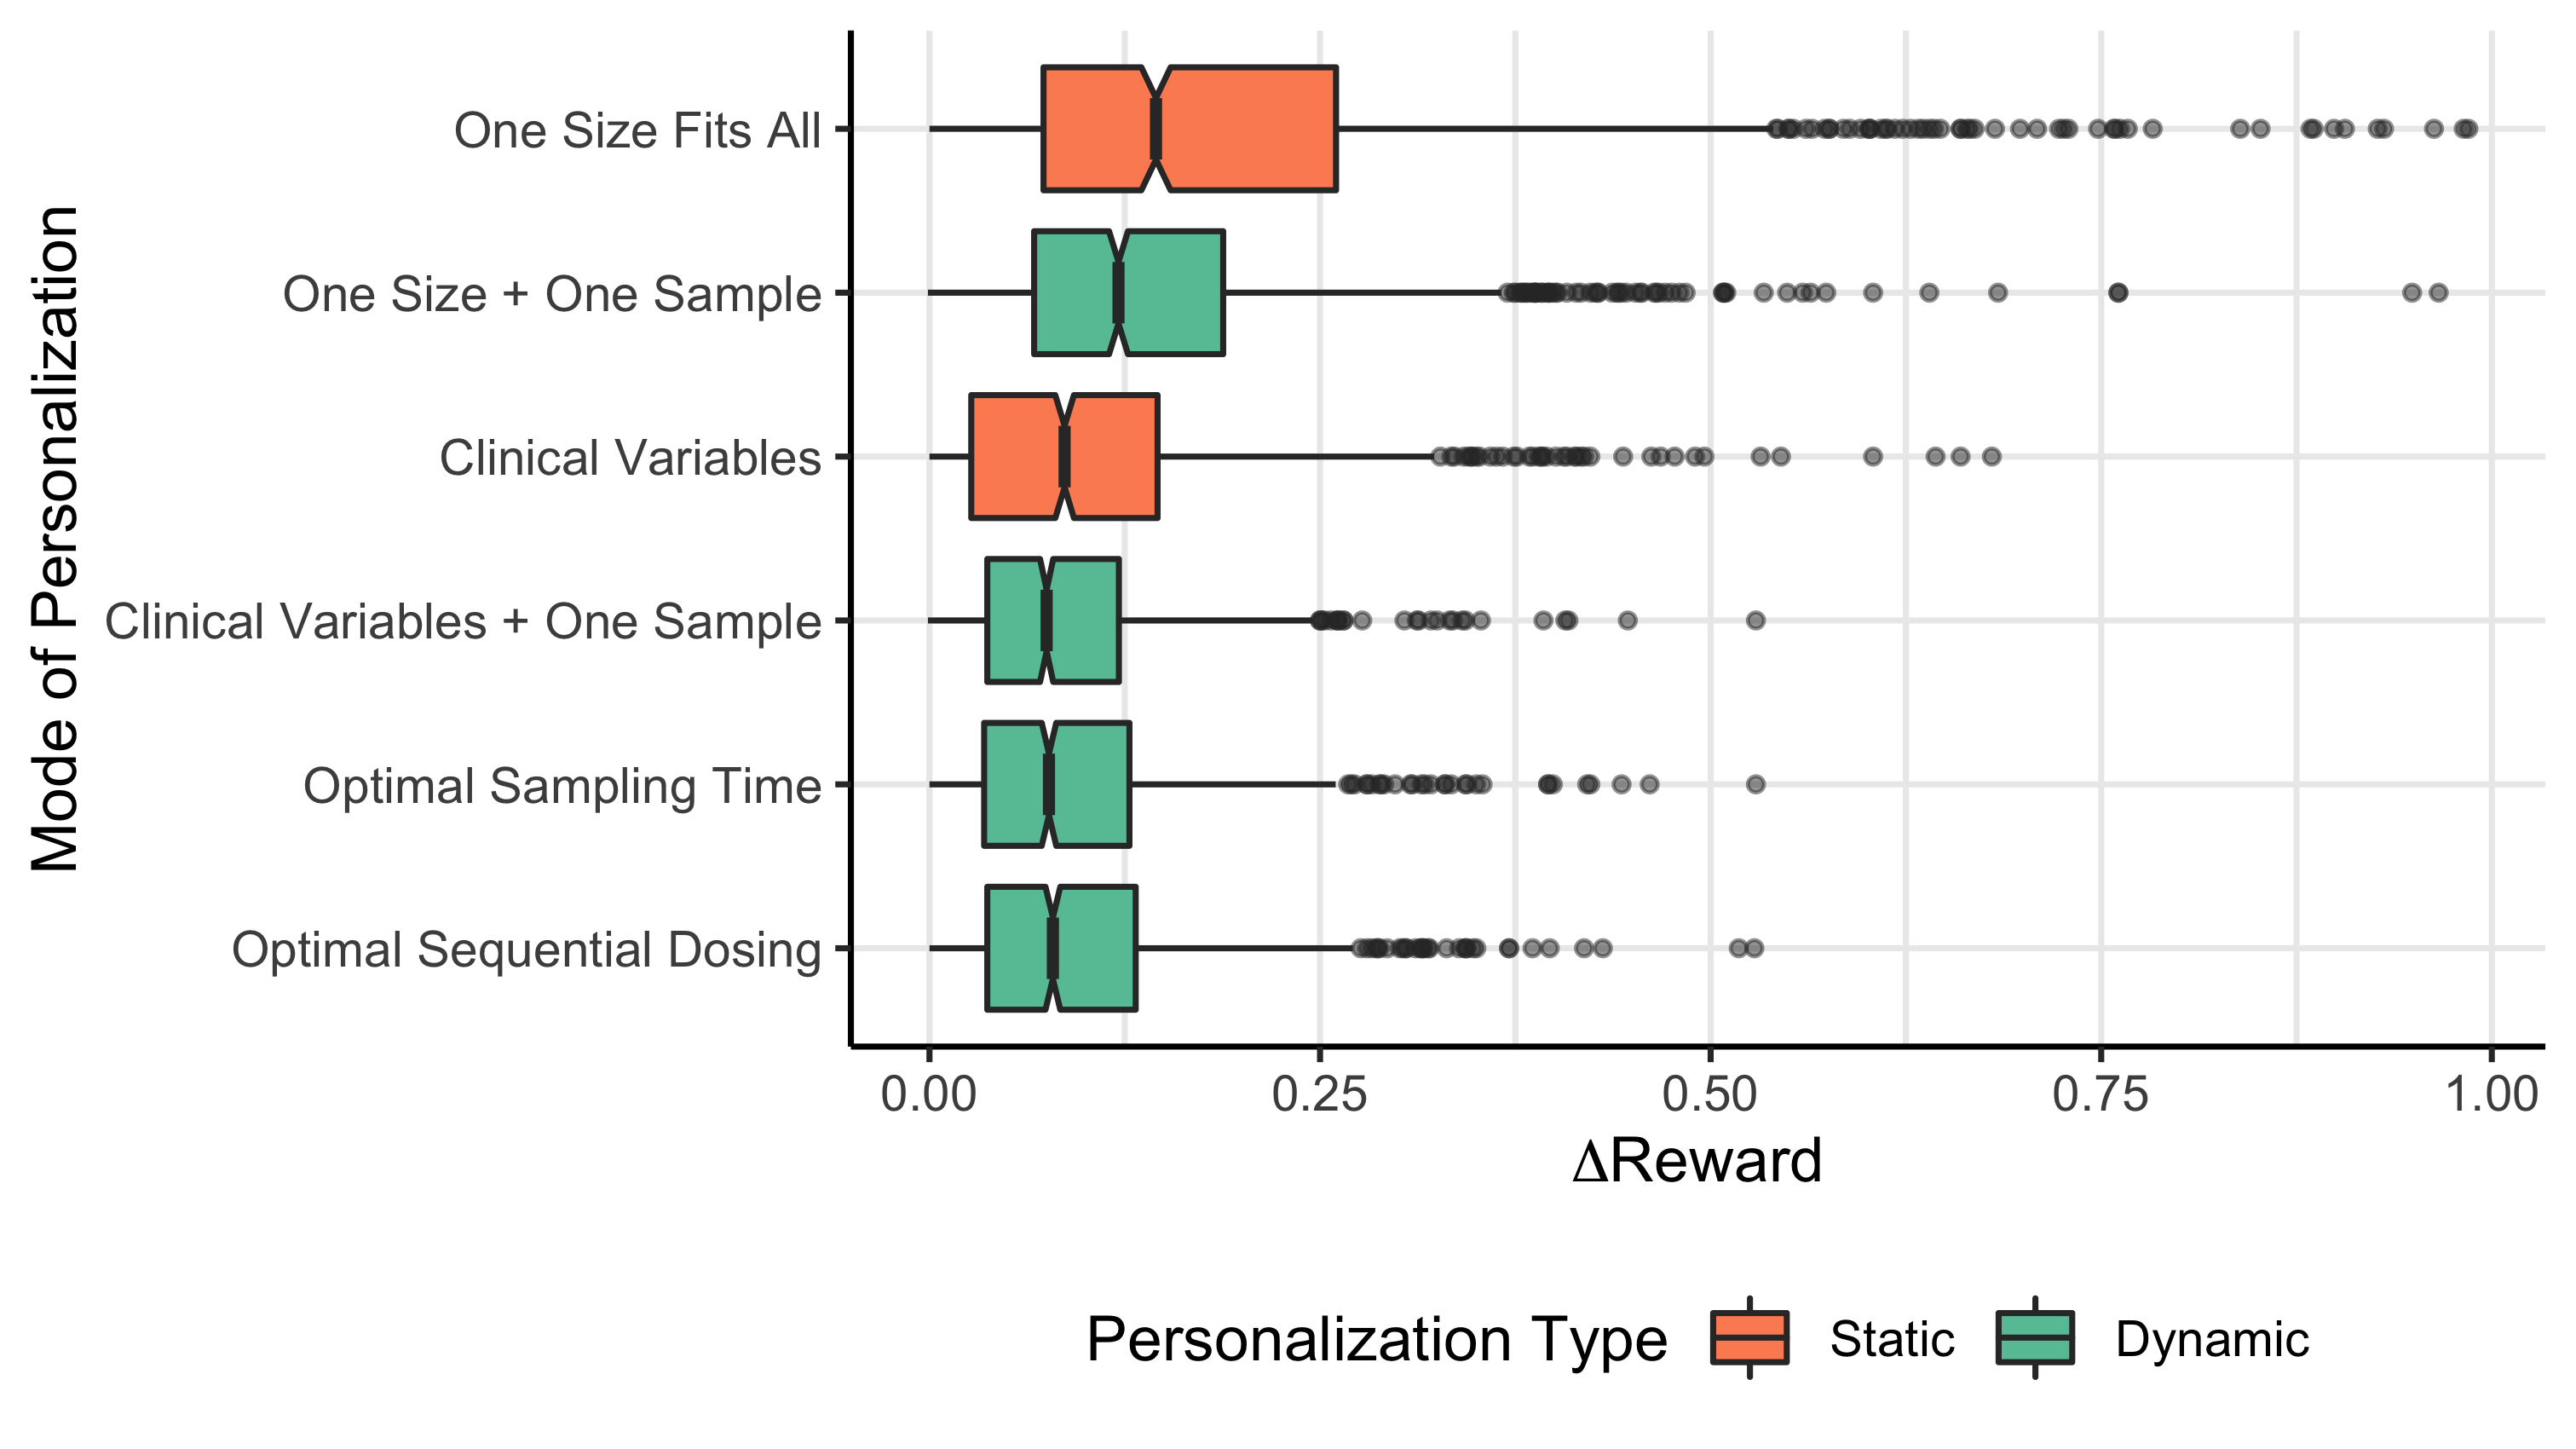
\includegraphics[width=1\linewidth]{figures/models_of_personalization_differences}
	\caption{Boxplots of the difference between theoretically largest reward and achieved reward for each of the 1000 simulated subjects. Subjects who achieve a reward close to their maximium reward have a difference on 0, subjects who achieve a reward less than their maximum have larger differences, with the largest difference being 1.}
	\label{fig:modelsofpersonalizationdifferences}
\end{figure}

	\section{Discussion}

Including age, sex, weight, and creatinine in our Bayesian model improved the inferences from that model.  Though the predicted concentrations and estimates of uncertainty changed negligibly, the covariates explained residual confounding in the random effects. This results in a model which better explains the observed variation in the data and hence should generate more plausible data for simulation.

That modes of personalization which use more information result in larger reward is ultimately unsurprising. From our perspective, the more pertinent result is the diminishing return on investment observed when using additional information (and consequently, taking on additional implementation burden to effectively use that information).  Were doses to be personalized for the simulated population, we would recommend the covariate model be used, as it is easier to implement, puts smaller burden on the clinic, and results in approximately mean/median rewards as compared to other methods.  Taking an additional sample doesn’t seem to improve the expected mean/median reward appreciably to be worth the burden of having the patient take time to come in, drawing their blood, measuring their concentration in the lab, and reporting results to the decision maker, in which a decision to not adjust the dose might be made anyway. Similar arguments can be made for Q learning, which has even higher implementation burden.

But mean/median reward does not tell the whole story.  As noted, the distribution of differences in reward is right skewed.  Some subjects have a very large difference, and the possibility of these differences might not be acceptable in different contexts with different drugs.  There is a tradeoff between less extreme differences and taking on additional clinic and implementation burden, and that tradeoff should be examined on a case by case basis.

Context is crucial, and how we adapt to that context is perhaps a question in need of closer examination.  Traditional methods of personalization include conditioning only on a subject’s covariates (not unlike the Covariate model we present here).  But of course patients are not their age, sex, weight, and creatinine.  Additionally, safety information and best available practices might change in the future as more research on drugs is performed. Were new safety information to be published, one might imagine the reward function might be affected, which may result in a new mode of personalization being more/less preferable or more/less feasible.  Any number of factors in flux can change the context in which personalization occurs, and that change in context may prompt for a re-evaluation in how personalization is done.

Thus, our results are not about apixaban per se.  We don’t offer recommendations on how personalization for apixaban should be done because we can’t anticipate the context.  What we offer is a framework for developing strategies of personalization and evaluating their performance against their implementation and clinic burden.  Context can be changed where needed, either through the reward function, or by adjusting when the clinic is able to take measurements, or by including additional information such as genotype in the Bayesian model.  Using this framework, clinics have flexibility to personalize the personalization.


\section{Limitations}

We’ve examined six modes for making decisions.  The next mode improves on a deficiency of the previous mode in a natural manner, and so our experiment constitutes a kind of ablation study.  We believe the decision making aspect of our study extracts information in a responsible way and uses the best decision making methodology available.  That being said, the experiment is not without limitations.

The bayesian model of the pharmacokinetics is integral to the methodology we present.  Any shortcomings in the model affect the quality of the decision and decision process.  Bayesian models are not as ubiquitous as other models in pharmacology, and so particular expertise is required for model development and evaluation.  That expertise increases the implementation burden of any decision process involving Bayesian models.  However, we demonstrate how one such model can be constructed in a past stdy [CITE] and include open sourced code and data for practitioners to replicate our model fitting.

Additionally, the data required to construct a high quality Bayesian model of pharmacokinetics require multiple observations of a single patient over an extended time, preferably over multiple well timed doses with near perfect adherence.  Obtaining such data requires well organized efforts and is high burden for both investigators and participating subjects.  This makes acquiring a robust Bayesian model for use in dose personalization difficult.

\section{Future Work}

Because the data required to build reliable Bayesian pharmacokinetic models are difficult to collect in practice, research into developing these models from observational data may prove fruitful in extending this work. If clinics record data on measured blood concentrations, they may have dozens or hundreds of subjects with only one or two measurements per subject.  Moreover, the subjects in question may be on multiple drugs or have comorbidities which may affect the pharmacokinetics of the drug under study.  Additional research into constructing Bayesian models which can adjust for polypharmacy and comorbidities while learning an individual’s pharmacokinetics from a large but sparse sample would drive this work towards being easier to implement in practice.



	\newpage
	\bibliography{./bibs/introduction,./bibs/dtr, ./bibs/bayes}

\end{document}